This chapter presents the results of the research in the thesis. For more information on how the data was collected, see Chapter \ref{Methodology}, Methodology. Firstly, optimal selections for each of the four projects will be presented to establish the benchmark for the ideal solution if the selection techniques choose perfectly. The goal is to find out which of the selection techniques; Size, Keyword, Cyclomatic Complexity, and Combination, is most effective in selecting the most important files for review.



\section{Optimal File Selection} \label{optimal_selections}
For each of the projects, there is a set of files that ideally should be selected for the technique to have made the \textit{correct} selections depending on which files are crucial to review. This is also important to ensure that the project is adequately covered in a code review. The relevant files vary for each project because they have been created by different student groups. The following subsections therefore presents the files that ideally should be selected for each technique to perform optimally. If the actual selection by the various techniques does not match the ideal selection, it could be due to several reasons. The primarily reason is, most probably, that the different selection techniques are not perfectly comprehensive and do not cover all aspects of the codebase. Additional information on the selection techniques can be found in Section \ref{Methodology}. \\

To establish a benchmark for evaluating the performance of each selection technique, I manually reviewed each of the projects to determine the optimal set of files. This process involved identifying the most crucial files that should be included in a thorough code review, considering factors such as functionality, complexity, size, critical features, and the amount of logic present. By creating a close-to-ideal selection scenario, it becomes easier to assess the strengths and weaknesses of each technique. In the following subsections, the files are presented along with the selection category they belong to. \\

This optimal selection process is based on my expertise and experience as a teaching assistant for three semesters, during which I reviewed numerous peer code submissions. The selected files are based on a combination of my understanding of the best practices in software development and my specific knowledge of the course projects. As mentioned above, the optimal selections are selected according to a combined assessment that considers functionality, complexity, size, critical features, and the amount of logic present. There is a degree of subjectivity in this selection, since it is merely my subjective opinions deciding what are crucial files to include. However, it provides an arguably reasonable standard that the automated selection techniques can be compared against. This selection process was completed before applying the various techniques to the projects so as not to be affected by their results and to keep the selection unbiased. \\

By comparing the files selected by each technique with this ideal set, we can identify where each method excels and where it does not suffice. This comparison will highlight the effectiveness of the different selection strategies in capturing the most crucial parts of the codebase, and will ensure that key functionalities are adequately reviewed. This analysis will provide valuable information on the practical application of these techniques in educational contexts.

\subsection{Project A - Optimal Selections}
For project A, the optimal selections are, ordered as they appear in the project, as follows: \\ 


\begin{center}
\begin{tabularx}{\textwidth}{>{\hsize=1.1\hsize}X >{\hsize=0.9\hsize}X}
    \toprule
    \textbf{Path} & \textbf{Selection Category} \\
    \midrule
    \texttt{src/resolvers.ts} & Functionality, Logic, Complexity  \\   
    \texttt{components/RecipeList/index.tsx} & Functionality, Logic, Complexity \\
    \texttt{components/RecipeListItem/index.tsx} & Logic \\   
    \texttt{components/Review/index.tsx} & Logic, Complexity \\
    \texttt{components/SearchBar/index.tsx} & Functionality \\
    \texttt{pages/MainPage/index.tsx} & Functionality,  Logic, Complexity \\
    \texttt{pages/RecipeDetails/index.tsx} & Functionality, Complexity \\
    \texttt{utils/GlobalContext.tsx} & Functionality, Logic\\
    \bottomrule
    
\end{tabularx}
\end{center}

\subsection{Project B - Optimal Selections}
For project B, the optimal selections are, ordered as they appear in the project, as follows: \\ 


\begin{center}
\begin{tabularx}{\textwidth}{>{\hsize=1.1\hsize}X >{\hsize=0.9\hsize}X}
    \toprule
    \textbf{Path} & \textbf{Selection Category} \\
    \midrule
    \texttt{backend/resolvers.ts} & Functionality,  Logic, Complexity  \\
    \texttt{components/DropdownMenu.tsx} & Logic, Complexity  \\
    \texttt{components/FavoriteButton.tsx} & Logic, Complexity  \\
    \texttt{components/Header.tsx} & Logic  \\
    \texttt{components/ReviewSection.tsx} & Functionality,  Logic, Complexity  \\
    \texttt{pages/Carpage.tsx} & Functionality,  Logic, Complexity  \\
    \texttt{pages/Filterpage.tsx} & Functionality,  Logic, Complexity  \\ 
    \texttt{pages/Homepage.tsx} & Functionality,  Logic  \\
    \bottomrule
\end{tabularx}
\end{center}


\subsection{Project C - Optimal Selections}
For project C, the optimal selections are, ordered as they appear in the project, as follows: \\ 


\noindent
\begin{center}
\begin{tabularx}{\textwidth}{>{\hsize=1.1\hsize}X >{\hsize=0.9\hsize}X}
    \toprule
    \textbf{Path} & \textbf{Selection Category} \\
    \midrule
    \texttt{Apollo-Server/index.tsx} & Functionality,  Logic, Complexity \\
    \texttt{Components/AboutWineComponent.tsx} & Functionality,  Logic, Complexity \\
    \texttt{Components/FilterComponent.tsx} & Functionality, Complexity \\
    \texttt{Components/HeaderComponent.tsx} & Functionality, Logic \\
    \texttt{Components/WineComponent.tsx} & Logic \\
    \texttt{pages/Homepage.tsx} & Functionality,  Logic, Complexity \\
    \texttt{contexts/FavoriteContext.tsx} & Functionality, Complexity \\
    \texttt{contexts/SearchContext.tsx} & Functionality \\
    \bottomrule
\end{tabularx}
\end{center}


\subsection{Control project - Optimal Selections}
For the control project, I could not confidently identify which files were more critical compared to the others, as it was such a complex project. Therefore, the files for these optimal selections are based solely on the various techniques. The comparison for this project in the discussion will not be compared to an optimal solution but instead will be all the selection techniques compared against each other for a joint comparison.\\




\section{Results for Each Selection Technique}
In this section, I will present the results for each of the file selections for each of the projects when applied with the different selection techniques. These selection techniques, presented in Section \ref{Methodology}, include Size Selection, Keyword Selection, Cyclomatic Complexity Selection, and Combination Selection. The results will highlight how well each technique identifies critical code segments and whether it aligns with the optimal selections presented in Section \ref{optimal_selections}. The files selected for each project will be visualized and then briefly described. This visualization will provide a detailed view of their performance. \\

To be able to visualize the results in a clear and organized manner, some adjustments have been made to the way the names of various files in the tables in this section are displayed. The files have been renamed to reflect the name of the folder above the file in the project hierarchy. For example, in table \ref{tab:Selected_files_A}, the name of \textit{Mainpage/index.tsx} has been changed to \textit{Mainpage.tsx}. For project C, some of the files with names containing "Component", have been renamed without that part. For example \textit{AboutWineComponent.tsx} to \textit{AboutWine.tsx}. This has no functional impact on the results or the thesis, but is solely to improve the presentation in the report.


\subsection{Project A Results}
For project A, the Keyword Selection technique only selected 7 files, although the specification was to select the 8 most crucial files. This is because the keywords selected to be searched for, which are introduced in Section \ref{Methodology}, only appeared in 7 of the files in the project. 


\begin{figure}[H]
  \centering
  \caption[Project A Selections and Metrics]{For each figure, the path to the selected file and the data point used to make the selection is shown. Figure (a) shows the files selected by the Size Selection technique, figure (b) shows the files selected by the Keyword Selection technique, figure (c) shows the files selected by the Cyclomatic Complexity Selection technique and figure (d) shows the files selected by the Combination Selection technique.}
  \subfloat[Selected files by Size Selection.]{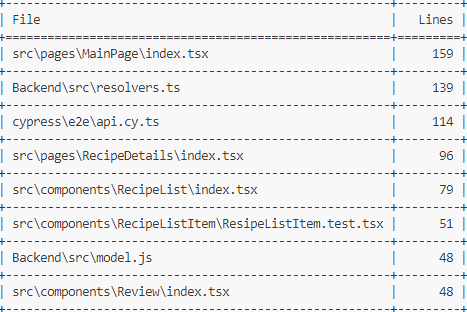
\includegraphics[width=0.49\textwidth]{Figures/A_Size.png}\label{fig:A_Size}}
  \hfill
  \subfloat[Selected files by Keyword Selection.]{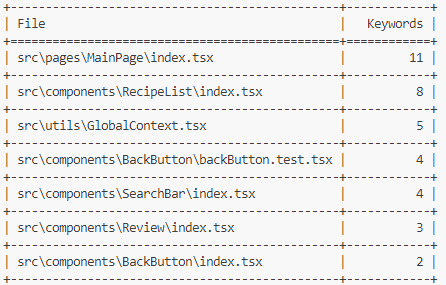
\includegraphics[width=0.46\textwidth]{Figures/A_Keyword.png}\label{fig:A_Keyword}}
  \hfill
  \subfloat[Selected files by Cyclomatic Complexity Selection.]{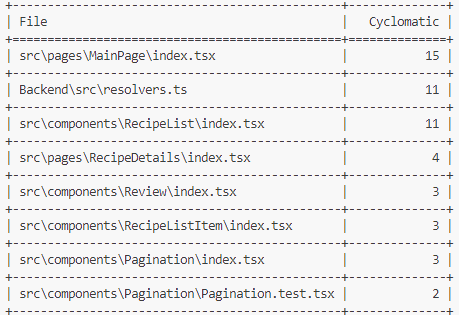
\includegraphics[width=0.49\textwidth]{Figures/A_Cyclomatic.png}\label{fig:A_Cyclomatic}}
  \hfill
  \subfloat[Selected files by Combination Selection.]{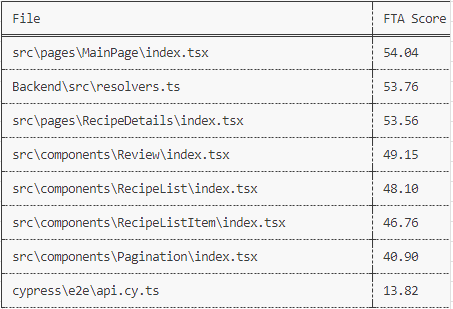
\includegraphics[width=0.49\textwidth]{Figures/A_Combination.png}\label{fig:A_Combination}}
  
\label{fig:Aresults}
\end{figure} \hfill 

The selected files by each technique have some overlap, which is both expected and a good indication that more than one selection technique effectively identifies crucial files.
The metric used by \textbf{Size Selection} selected files ranging from 159 to 48 lines of code (LOC), meaning that the following files after the 8 selected by this technique had equal or even fewer LOC and therefore probably had less relevance for being selected for review.
The metric selected for \textbf{Keyword Selection} were "useState", "useEffect", and "useNavigate", and were present in 7 of the files in project A. This metric ranged from 11 cases in \textit{Mainpage.tsx} to 2 cases in \textit{BackButton.tsx}.
The \textbf{Cyclomatic Complexity} metric ranged from a score of 15 in \textit{Mainpage.tsx} to 2 in \textit{Pagination.test.tsx}.
In the results from \textbf{Combination Selection}, the FTA scores ranged from 54.04 in \textit{Mainpage.tsx} to 13.82 in \textit{Pagination.tsx}. However, it should be noted that the seventh selection in the Combination Selection had an FTA score of 40.90. This indicates that the first 7 files selected by this technique covered the most problematic files which subsequently would be the most relevant ones for review. \\

Table \ref{tab:Selected_files_A} below visualizes the files selected by each technique with colors showing the corresponding selections between the different selection techniques.

\begin{table}[h!]
  \centering
  \fontsize{10}{10}\selectfont
  \caption{Comparison of selected files for project A by each technique}
  \label{tab:Selected_files_A}
  \begin{tabularx}{\textwidth}{llll}
    \hline
     \textbf{Size} & \textbf{Keyword} & \textbf{Cyclomatic } & \textbf{Combination} \\
     \textbf{} & \textbf{} & \textbf{Complexity } & \textbf{} \\ [1ex] \hline \hline 
    \colorbox{BurntOrange}{Mainpage.tsx} & \colorbox{BurntOrange}{MainPage.tsx} & \colorbox{BurntOrange}{MainPage.tsx} & \colorbox{BurntOrange}{MainPage.tsx} \\ [2ex]
    \colorbox{Tan}{resolvers.ts} & \colorbox{PineGreen}{RecipeList.tsx} & \colorbox{Tan}{resolvers.ts} & \colorbox{Tan}{resolvers.ts} \\ [2ex]
    \colorbox{WildStrawberry}{api.cy.ts} & GlobalContext.tsx & \colorbox{PineGreen}{RecipeList.tsx} & \colorbox{CornflowerBlue}{RecipeDetails.tsx} \\ [2ex]
    \colorbox{CornflowerBlue}{RecipeDetails.tsx} & backButton.test.tsx & \colorbox{CornflowerBlue}{RecipeDetails.tsx} & \colorbox{Rhodamine}{Review.tsx} \\ [2ex] 
    \colorbox{PineGreen}{RecipeList.tsx} & SearchBar.tsx & \colorbox{Rhodamine}{Review.tsx} & \colorbox{PineGreen}{RecipeList.tsx} \\ [2ex] 
    ResipeListItem.test.tsx & \colorbox{Rhodamine}{Review.tsx} & \colorbox{Mulberry}{RecipeListItem.tsx} & \colorbox{Mulberry}{RecipeListItem.tsx} \\ [2ex] 
    model.js & Backbutton.tsx & \colorbox{LimeGreen}{Pagination.tsx} & \colorbox{LimeGreen}{Pagination.tsx} \\ [2ex]
    \colorbox{Rhodamine}{Review.tsx} & ----------------- & Pagination.test.tsx & \colorbox{WildStrawberry}{api.cy.ts} \\ [2ex] 

  \end{tabularx}
\end{table}


For project A, the different techniques had some overlap in the selected files. All techniques selected \textit{MainPage.tsx} as the most critical file to be reviewed. After this, only Keyword Selection did not have \textit{resolvers.ts} as the second most crucial; in fact, this file was not present in its selections at all. \\

From here, the various techniques started differentiating more in the ordering of importance of files for review. However, the selected files by Size, Cyclomatic Complexity, and Combination Selection were about the same with a few exceptions. These were that Size Selection was the only technique that selected \textit{ResipeListItem.test.tsx} and \textit{model.js}, while Cyclomatic Complexity Selection was the only technique that selected \textit{Pagination.test.tsx}. \\

Combination Selection was the only technique that had all its files selected by at least one other technique, while Keyword Selection had the most files solely selected by this technique. There were two files selected uniquely by Size Selection that were not selected by any other technique. This applied to four files for Keyword Selection and one file for Cyclomatic Complexity.



\newpage
\subsection{Project B Results} 
The selections for each technique applied in project B are shown in Figure \ref{fig:Bresults}. 

\begin{figure}[H]
  \centering
  \caption[Project B Selections and Metrics]{For each figure, the path to the selected file and the data point used to make the selection is shown. Figure (a) shows the files selected by the Size Selection technique, figure (b) shows the files selected by the Keyword Selection technique, figure (c) shows the files selected by the Cyclomatic Complexity Selection technique and figure (d) shows the files selected by the Combination Selection technique.}
  \subfloat[Selected files by Size Selection.]{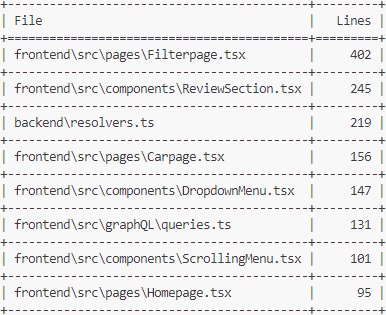
\includegraphics[width=0.47\textwidth]{Figures/B_Size.png}\label{fig:B_Size}}
  \hfill
  \subfloat[Selected files by Keyword Selection.]{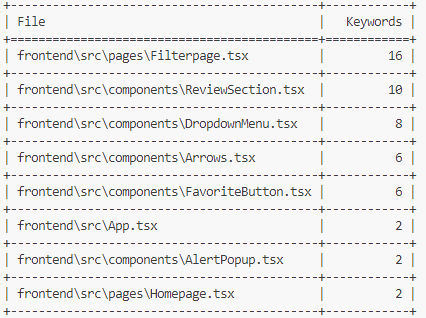
\includegraphics[width=0.51\textwidth]{Figures/B_Keyword.png}\label{fig:B_Keyword}}
  \hfill
  \subfloat[Selected files by Cyclomatic Complexity Selection.]{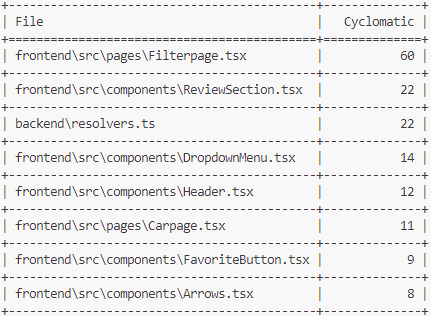
\includegraphics[width=0.49\textwidth]{Figures/B_Cyclomatic.png}\label{fig:B_Cyclomatic}}
  \hfill
  \subfloat[Selected files by Combination Selection.]{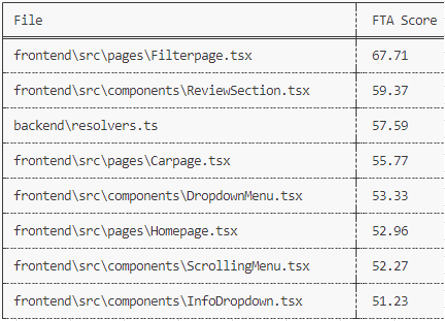
\includegraphics[width=0.49\textwidth]{Figures/B_Combination.png}\label{fig:B_Combination}}
  
\label{fig:Bresults}
\end{figure} \hfill 

Similarly as with project A, the selected files by each technique have some overlap, which was both expected, and also a good indication that more than one selection technique effectively identifies which files are crucial. 
For project B, the metric used by \textbf{Size Selection} selected files that ranged from 402 to 95 lines of code (LOC). This is a larger gap than for project A. In addition, the eighth file having 95 LOC could indicate that the following files after this would also have code that might be necessary to include in a review.
The metrics selected for \textbf{Keyword Selection} were present in 9 of the files in project B. This metric ranged from 16 cases in \textit{Filterpage.tsx} to 2 cases in \textit{Homepage.tsx}.
The \textbf{Cyclomatic Complexity} metric ranged from a score of 60 in \textit{Filterpage.tsx} to 8 in \textit{Arrows.tsx}. This represents a significant increase compared to project A, which had a Cyclomatic Complexity score of 15 in \textit{Mainpage.tsx}.
In the results from the \textbf{Combination Selection}, the FTA scores ranged from 67.71 in \textit{Filterpage.tsx} to 51.23 in \textit{InfoDropdown.tsx}. After the 15th file selection with Combination Selection, the FTA score went from 46.43 in one file to 12.73 for the next.


\begin{table}[h!]
  \centering
  \fontsize{10}{10}\selectfont
  \caption{Comparison of selected files for project B by each technique}
  \label{tab:Selected_files_B}
  \begin{tabularx}{\textwidth}{llll}
    \hline
     \textbf{Size} & \textbf{Keyword} & \textbf{Cyclomatic } & \textbf{Combination} \\
     \textbf{} & \textbf{} & \textbf{Complexity } & \textbf{} \\ [1ex] \hline \hline 
    \colorbox{BurntOrange}{Filterpage.tsx} & \colorbox{BurntOrange}{Filterpage.tsx} & \colorbox{BurntOrange}{Filterpage.tsx} & \colorbox{BurntOrange}{Filterpage.tsx} \\ [2ex]
    \colorbox{Tan}{ReviewSection.tsx} & \colorbox{Tan}{ReviewSection.tsx} & \colorbox{Tan}{ReviewSection.tsx} & \colorbox{Tan}{ReviewSection.tsx} \\ [2ex]
    \colorbox{CornflowerBlue}{resolvers.ts} & \colorbox{PineGreen}{DropdownMenu.tsx} & \colorbox{CornflowerBlue}{resolvers.ts} & \colorbox{CornflowerBlue}{resolvers.ts} \\ [2ex]
    \colorbox{Rhodamine}{Carpage.tsx} & \colorbox{WildStrawberry}{Arrows.tsx} & \colorbox{PineGreen}{DropdownMenu.tsx} & \colorbox{Rhodamine}{Carpage.tsx} \\ [2ex] 
    \colorbox{PineGreen}{DropdownMenu.tsx} & \colorbox{Orchid}{FavoriteButton.tsx} & Header.tsx & \colorbox{PineGreen}{DropdownMenu.tsx} \\ [2ex] 
    queries.ts & App.tsx & \colorbox{Rhodamine}{Carpage.tsx} & \colorbox{Mulberry}{Homepage.tsx} \\ [2ex] 
    \colorbox{LimeGreen}{ScrollingMenu.tsx} & AlertPopup.tsx & \colorbox{Orchid}{FavoriteButton.tsx} & \colorbox{LimeGreen}{ScrollingMenu.tsx} \\ [2ex]
    \colorbox{Mulberry}{Homepage.tsx} & \colorbox{Mulberry}{Homepage.tsx} & \colorbox{WildStrawberry}{Arrows.tsx} & InfoDropdown.tsx \\ [2ex] 

  \end{tabularx}
\end{table}

Also in project B there was overlap in the most crucial files identified by each technique. All selection techniques had selected the two same files as the most crucial and second most crucial. These files were \textit{Filterpage.tsx} and \textit{ReviewSection.tsx} respectively. All techniques had also selected \textit{DropdownMenu.tsx}, but with a difference in the ordering of importance. \\

After this point, the various techniques had some overlap with other techniques in most of the selections. Size Selection and Combination Selection had the most in common, with both having only one selection, which the other did not. Keyword Selection and Cyclomatic Complexity Selection also had more selections in common than the other two. They had two file selections in common that the other techniques did not select, specifically \textit{Arrows.tsx} and \textit{FavoriteButtion.tsx}. \\

For project B, all the selection techniques had at least one selection that no other technique had selected. For Size Selection it was \textit{queries.ts}, for Keyword Selection it was \textit{App.tsx} and \textit{AlertPopup.tsx}, for Cyclomatic Complexity Selection it was \textit{Header.tsx} while for Combination Selection it was \textit{InfoDropdown.tsx}. \\




\subsection{Project C Results} 

\begin{figure}[H]
  \centering
  \caption[Project C Selections and Metrics]{For each figure, the path to the selected file and the data point used to make the selection is shown. Figure (a) shows the files selected by the Size Selection technique, figure (b) shows the files selected by the Keyword Selection technique, figure (c) shows the files selected by the Cyclomatic Complexity Selection technique and figure (d) shows the files selected by the Combination Selection technique.}
  \subfloat[Selected files by Size Selection.]{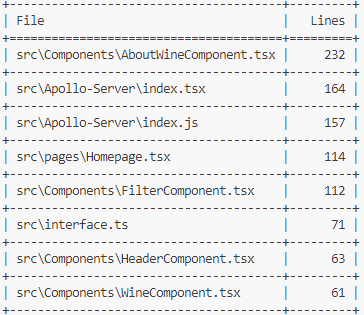
\includegraphics[width=0.48\textwidth]{Figures/C_Size.png}\label{fig:C_Size}}
  \hfill
  \subfloat[Selected files by Keyword Selection.]{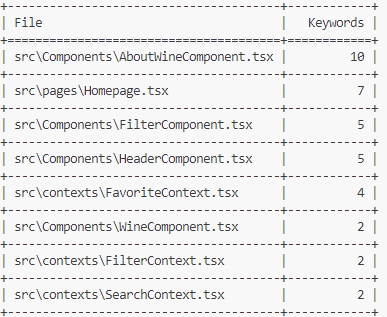
\includegraphics[width=0.50\textwidth]{Figures/C_Keyword.png}\label{fig:C_Keyword}}
  \hfill
  \subfloat[Selected files by Cyclomatic Complexity Selection.]{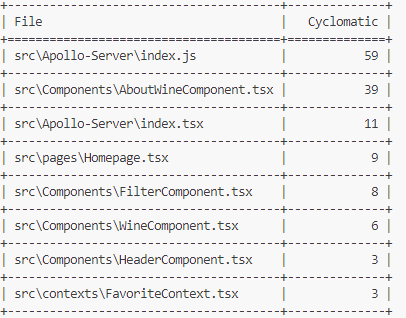
\includegraphics[width=0.51\textwidth]{Figures/C_Cyclomatic.png}\label{fig:C_Cyclomatic}}
  \hfill
  \subfloat[Selected files by Combination Selection.]{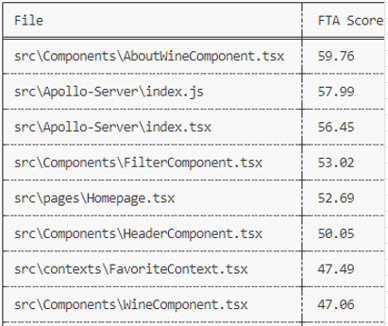
\includegraphics[width=0.48\textwidth]{Figures/C_Combination.png}\label{fig:C_Combination}}
  
\label{fig:Cresults}
\end{figure} \hfill 

In project C, the metric used by \textbf{Size Selection} selected files ranging from 232 LOC to 61 LOC. This is more similar to the gap found in project A. However, since the eighth file had 61 LOC, it is possible that there are crucial files below this threshold as well that were excluded selection.
In this project, \textbf{Keyword Selection} found the selected keywords in 10 files. These cases ranged from 10 occurrences in \textit{AboutWine.tsx} to two occurrences in \textit{Favoritepage.tsx}.
\textbf{Cyclomatic Complexity Selection} ranged from a score of 59 in \textit{Apollo-Server.tsx} to a score of three in \textit{FavoriteContext.tsx}. This was similar to the result from applying this technique on project B, but in this instance it selected all the files with a score above three instead.
The \textbf{Combination Selection} had files selected with scores ranging from 59.76 to 47.06 in \textit{AboutWine.tsx} to \textit{Wine.tsx} respectively. The FTA score dropped to 12.56 with the file following \textit{Wine.tsx}, indicating that the first eight files clearly were the most crucial ones. \\


\begin{table}[H]
  \centering
  \fontsize{10}{10}\selectfont
  \caption{Comparison of selected files for project C by each technique}
  \label{tab:Selected_files_C}
  \begin{tabularx}{\textwidth}{llll}
    \hline
     \textbf{Size} & \textbf{Keyword} & \textbf{Cyclomatic } & \textbf{Combination} \\
     \textbf{} & \textbf{} & \textbf{Complexity } & \textbf{} \\ [1ex] \hline \hline 
    \colorbox{BurntOrange}{AboutWine.tsx} & \colorbox{BurntOrange}{AboutWine.tsx} & \colorbox{Tan}{Apollo-Server.js} & \colorbox{BurntOrange}{AboutWine.tsx} \\ [2ex]
    \colorbox{CornflowerBlue}{Apollo-Server.tsx} & \colorbox{Rhodamine}{Homepage.tsx} & \colorbox{BurntOrange}{AboutWine.tsx} & \colorbox{Tan}{Apollo-Server.js} \\ [2ex]
    \colorbox{Tan}{Apollo-Server.js} & \colorbox{PineGreen}{Filter.tsx} & \colorbox{CornflowerBlue}{Apollo-Server.tsx} & \colorbox{CornflowerBlue}{Apollo-Server.tsx} \\ [2ex]
    \colorbox{Rhodamine}{Homepage.tsx} & \colorbox{LimeGreen}{Header.tsx} & \colorbox{Rhodamine}{Homepage.tsx} & \colorbox{PineGreen}{Filter.tsx} \\ [2ex] 
    \colorbox{PineGreen}{Filter.tsx} & \colorbox{Orchid}{FavoriteContext.tsx} & \colorbox{PineGreen}{Filter.tsx} & \colorbox{Rhodamine}{Homepage.tsx} \\ [2ex] 
    interface.ts & \colorbox{Mulberry}{Wine.tsx} & \colorbox{Mulberry}{Wine.tsx} & \colorbox{LimeGreen}{Header.tsx} \\ [2ex] 
    \colorbox{LimeGreen}{Header.tsx} & FilterContext.tsx & \colorbox{LimeGreen}{Header.tsx} & \colorbox{Orchid}{FavoriteContext.tsx} \\ [2ex]
    \colorbox{Mulberry}{Wine.tsx} & SearchContext.tsx & \colorbox{Orchid}{FavoriteContext.tsx} & \colorbox{Mulberry}{Wine.tsx} \\ [2ex] 

  \end{tabularx}
\end{table}

Project C is the one with the most crucial file selection overlap of the three test projects. As seen in Table \ref{tab:Selected_files_C}, there are only three selected files that were selected by a single technique. These files were \textit{interface.ts} which got selected by Size Selection, and \textit{FilterContext.tsx} and \textit{SearchContext.tsx} which got selected by Keyword Selection. All remaining selected files were selected by at least one other technique. \\

Size, Cyclomatic Complexity, and Combination Selection all selected the same files as the 5 most crucial files. However, they all had different placements in the order of importance. The only similar ordering was \textit{Homepage.tsx} and \textit{Filter.tsx} for Size and Cyclomatic Complexity, and \textit{Apollo-Server.tsx} for Cyclomatic Complexity and Combination. \\

For this project, Cyclomatic Complexity Selection and Combination Selection had selected all the same files, just with different ordering. Size Selection selected one different file, which exempted it from having identical selections to Cyclomatic Complexity and Combination. \\



\subsection{Control Project Results} 
The control project serves as a benchmark to evaluate the performance of each selection technique on a larger and more complex codebase. The following subsection details the results of applying each technique in this project.

\begin{figure}[H]
  \centering
  \caption[Control Project Selections and Metrics]{For each figure, the path to the selected file and the data point used to make the selection. Figure (a) shows the files selected by the Size Selection technique, figure (b) shows the files selected by the Keyword Selection technique, figure (c) shows the files selected by the Cyclomatic Complexity Selection technique and figure (d) shows the files selected by the Combination Selection Technique.}
  \subfloat[Selected files by Size Selection.]{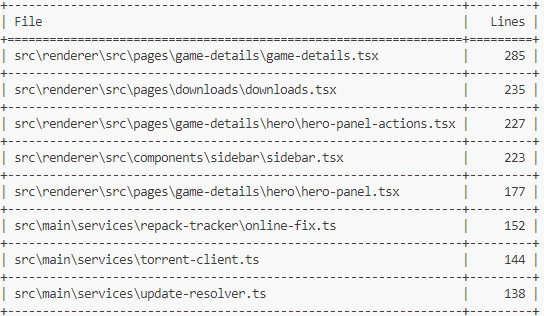
\includegraphics[width=0.48\textwidth]{Figures/Control_Size.png}\label{fig:Control_Size}}
  \hfill
  \subfloat[Selected files by Keyword Selection.]{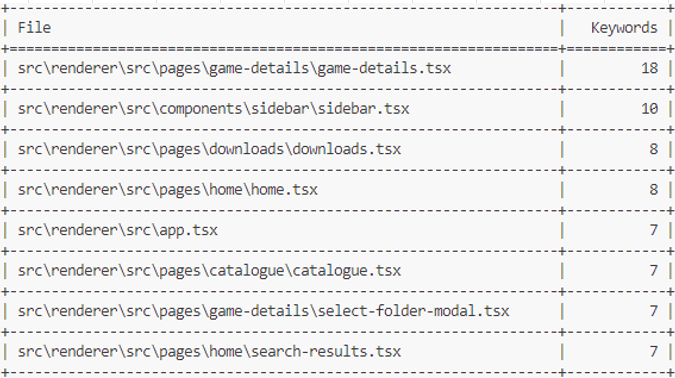
\includegraphics[width=0.48\textwidth]{Figures/Control_Keyword.png}\label{fig:Control_Keyword}}
  \hfill
  \subfloat[Selected files by Cyclomatic Complexity Selection.]{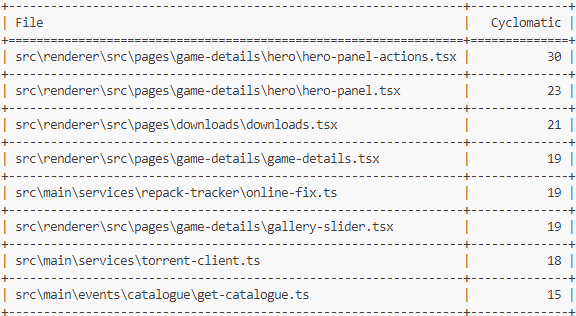
\includegraphics[width=0.54\textwidth]{Figures/Control_Cyclomatic.png}\label{fig:Control_Cyclomatic}}
  \hfill
  \subfloat[Selected files by Combination Selection.]{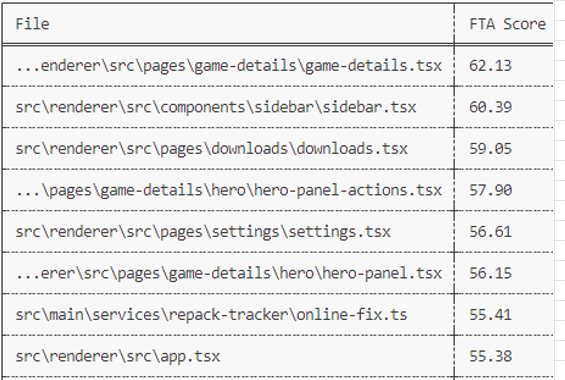
\includegraphics[width=0.44\textwidth]{Figures/Control_Combination.png}\label{fig:Control_Combination}}
  \label{fig:Controlresults}
\end{figure}

We can see that the selected files for each technique have some overlap, although not as much as the test projects. This is not surprising, as the codebase in this control project is both bigger and more complex than the test projects.
The \textbf{Size Selection} technique this time selected files with metrics ranging from 285 lines of code in \textit{game-details.tsx} to 138 lines of code in \textit{update-resolver.ts}. 
As a substantially larger project, this time the \textbf{Keyword Selection} found keywords in 22 files, which is more than twice the amount found in any test project. The occurrences ranged from 18 in \textit{game-details.tsx} to 7 occurrences in \textit{search-result.tsx}, and down to 2 in the least prioritized file.
The \textbf{Cyclomatic Complexity Selection} metric ranged from 30 in \textit{hero-panel-actions.tsx} to a score of 15 in \textit{get-catalogue.tsx}. 
\textbf{Combination Selection} this time ranged from a FTA score in \textit{game-details.tsx} of 62.13 to \textit{app.tsx} with a FTA score of 55.38. In the control project, the FTA score was above 30 all the way until the 55th file selection, then it dropped to 14 and below. This indicates that most of the files until this 55th file could be relevant to include in a review. \\


\begin{table}[H]
  \centering
  \caption{Comparison of selected files for control project by each technique}
  \label{tab:Selected_files_control}
  \begin{tabularx}{\textwidth}{llll}
    \hline
     \textbf{Size} & \textbf{Keyword} & \textbf{Cyclomatic } & \textbf{Combination} \\
     \textbf{} & \textbf{} & \textbf{Complexity } & \textbf{} \\ [1ex] \hline \hline 
    \colorbox{BurntOrange}{game-details.tsx} & \colorbox{BurntOrange}{game-details.tsx} & \colorbox{Rhodamine}{hero-actions.tsx} & \colorbox{BurntOrange}{game-details.tsx} \\ [2ex]
    \colorbox{Tan}{downloads.tsx} & \colorbox{CornflowerBlue}{sidebar.tsx} & \colorbox{PineGreen}{hero-panel.tsx} & \colorbox{CornflowerBlue}{sidebar.tsx} \\ [2ex]
    \colorbox{Rhodamine}{hero-actions.tsx} & \colorbox{Tan}{downloads.tsx} & \colorbox{Tan}{downloads.tsx} & \colorbox{Tan}{downloads.tsx} \\ [2ex]
    \colorbox{CornflowerBlue}{sidebar.tsx} & home.tsx & \colorbox{BurntOrange}{game-details.tsx} & \colorbox{Rhodamine}{hero-actions.tsx} \\ [2ex] 
    \colorbox{PineGreen}{hero-panel.tsx} & \colorbox{WildStrawberry}{app.tsx} & \colorbox{Mulberry}{online-fix.ts} & settings.tsx \\ [2ex] 
    \colorbox{Mulberry}{online-fix.ts} & catalogue.tsx & gallery-slider.tsx & \colorbox{PineGreen}{hero-panel.tsx} \\ [2ex] 
    \colorbox{LimeGreen}{torrent-client.ts} & select-modal.tsx & \colorbox{LimeGreen}{torrent.client.ts} & \colorbox{Mulberry}{online-fix.ts} \\ [2ex]
    update-resolver.ts & search-results.tsx & get-catalogue.ts & \colorbox{WildStrawberry}{app.tsx} \\ [2ex] 

  \end{tabularx}
\end{table}

In the control project, there were more notable differences between the various techniques than in the test projects. Although, there was still some overlap in the selections, such as all techniques choosing \textit{game-details.tsx} and \textit{downloads.tsx} among the most important files. However, Cyclomatic Complexity stood out in this by indicating that \textit{downloads.tsx} was more important than \textit{game-details.tsx}. At the same time, the other three techniques had chosen \textit{sidebar.tsx} among the most important files, while Cyclomatic Complexity did not select it. \\

Keyword Selection had the most different selections compared to the other techniques, with only 4 out of 8 files being chosen by at least one other technique. It did not select files such as \textit{hero-panel-actions.tsx}, \textit{online-fix.tsx}, and \textit{hero-panel.tsx}, which the other three techniques all selected. \\

The Control Project and Project C were the projects in which all techniques had selected at least one file exclusively that none of the other techniques had selected. For this project, it was one file for Size Selection, four files for Keyword Selection, two files for Cyclomatic Complexity Selection, and one file for Combination Selection.